\documentclass{article}

\usepackage{mhchem}
\usepackage{siunitx}
\usepackage{graphicx}
\usepackage{caption}

\newcommand{\cc}{$\,\text{cm}^{3}$}
\newcommand{\circa}{\emph{circa }}
\newcommand{\g}{\,g}

\title{Experiment 1}
\date{01/12/2020}
\author{Samuel J. Frost -- pcysf6}

\begin{document}

\maketitle

\section*{Synthesis}
\subsection*{Part 1 --- Synthesis of \ce{[NiCl2(PPh3)2]}}
\ce{NiCl2.6H2O} (0.66\g, 2.77\,mmol) was dissolved in ethanol (12\cc) and warmed to \circa \SI{40}{\celsius} to give a green solution.
Triphenylphosphine (1.55\g, 5.9\,mmol) was suspended in propan-2-ol (20\cc) and refluxed until fully dissolved.
The warm nickel chloride solution was added down the condenser dropwise. The solution was refluxed for 
20 minutes and then allowed to cool to room temperature. The product was isolated via vacuum filtration,
washed with warm propan-2-ol (20\cc) and cold diethyl ether (10\cc). The product was allowed to dry giving a red powder.
 (1.24\g, 68\,\%)

\subsection*{Part 2 --- Synthesis of \ce{[Ni(NCS)2(PPh3)2]}}
\ce{Ni(NO3)2.6H2O} (0.77\g, 2.64\,mmol) was dissolved in ethanol (20\cc). Potassium thiocyanate (0.52\g, 5.36\,mmol)
was ground and added to the solution and then refluxed for 20 minutes. The solution was cooled on ice and 
then collected under gravity filtration. The solution was warmed to \circa \SI{40}{\celsius}.

Triphenylphosphine (1.42\g, 5.42\,mmol) was added to propan-2-ol (20\cc) and refluxed until the
triphenylphosphine had dissolved. The nickel thiocyanate solution was added dropwise into the condenser and then
refluxed for a further 15 minutes. The solution was cooled to room temperature and the product isolated via vacuum filtration.
The product was washed with warm propan-2-ol (20\cc) and cold diethyl ether (10\cc). The product was dried on the 
filter giving a black powder. (0.41\g, 22\,\%)

\newpage
\section*{Analysis}
Both products were analysed via a UV spectrum 

\begin{figure}[h]
    \centering
    \captionsetup{justification=centering}
    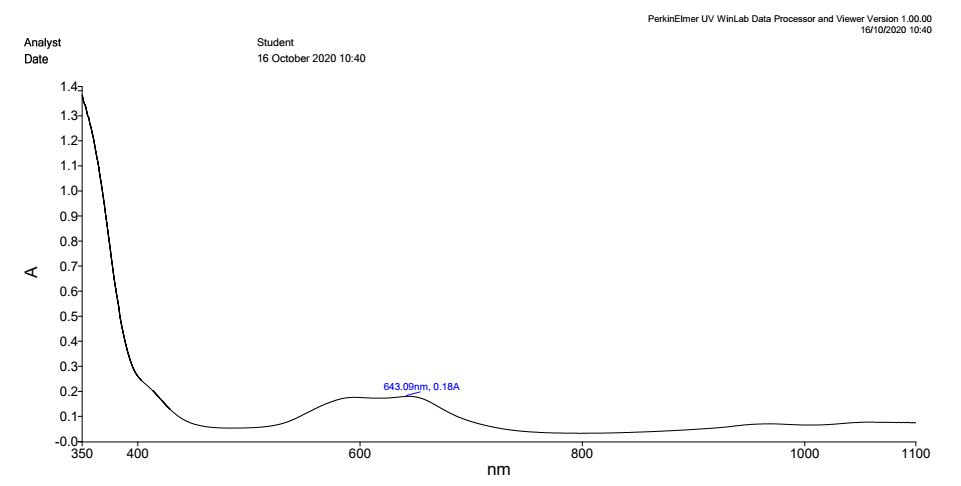
\includegraphics[width=\textwidth, height=\textheight, keepaspectratio]{cl.jpg}
    \caption{UV spectrum of \ce{[NiCl2(PPh3)2]} in a soltion of dichloromethane}
\end{figure}

\begin{figure}[h]
    \centering
    \captionsetup{justification=centering}
    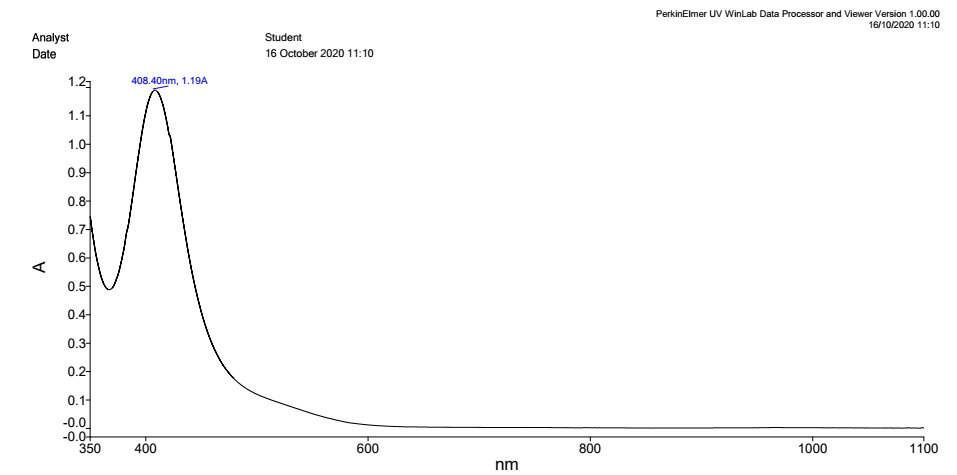
\includegraphics[width=\textwidth, height=\textheight, keepaspectratio]{nc.jpg}
    \caption{UV spectrum of \ce{[Ni(NCS)2(PPh3)2]} in a solution of acetonitrile}
\end{figure}

\end{document}